\chapter{Theoretical and Conceptual Frameworks}\label{ch:tf-cf}
The theories from the literatures reviewed in the preceding chapter will be discussed in this chapter. In addition to this, the solutions will be presented at a high level through the conceptual framework, where the details will be discussed in the methodologies.
\section{Theoretical Framework}
As mentioned from Chapter \ref{ch:rrl}, when it comes to statistical analyses of the morphological characteristics of the Qur'\=an corpus \shortcite{dukes-habash-2010-morphological}, most of it were simply comparison to the other corpora, none has yet looked into it in terms of statistical analyses of the positional statistics of these morphological features like the parts-of-speech, and name of entities like God's names and prophets names. The interest in studying this statistics will also help in understanding the structure of the Qur'\=an as it should give us an idea on how these topics or names of these entities are positioned in the Qur'\=an.

Moreover, in Chapter \ref{ch:rrl}, the work of \shortciteA{siddiqui2013} used Latent Dirichlet Allocation (LDA) on 24 \arb[trans]{sUwar} \arb{sUwar} using Term Frequency-Inverse Document Frequency (TF-IDF) as the word embeddings. While this procedure does work, but the recent development on Large Language Models (LLMs) has resulted into improved word embeddings, such as the Bidirectional Encoding Representation from Transformers (BERT) models \shortcite{devlin2018bert}. BERT models, discussed in Section \ref{sec:bert}, are superior than TF-IDF since, by design, it has lower dimensional embedding and does not depend on the number of vocabularies. Semantically, it is also better as it uses a \textit{attention mechanism}\footnote{\textit{See} Section \ref{sec:attention-mechanism}}, which takes into account the surrounding contexts of the given embedding. Further, while LDA is an effective statistical methodology for topic modeling, this paper will also look into BERTopic by \shortciteA{grootendorst2022bertopic}, which is a topic modeling model based on BERT and was found to provide better results compared to other algorithms according to \shortciteA{egger2022topic}.

Further, when it comes to \textit{rhythmic analyses} of the Qur'\=an's texts, none so far has looked into it from the perspective of statistical analyses. As such, this paper will also provide a mathematical formulation of the said analyses, and also its applications to statistical methodologies. This is the first to do so, and methods for this analyses will include cluster analyses to understand if there are groupings of \arb[trans]{sUwar} \arb{sUwar} with respect to this statistics, and also \textit{discrete-time markov chain} to study the transition probabilities of the changes in the rhythmic syllables of the Qur'\=an.  Other methodologies will revolve around descriptive statistics to describe the rhythmic signatures of \arb[trans]{sUwar} \arb{sUwar} with respect to its place of revelation, that is, either \arb[trans]{makkiyyaT} \arb{makkiyyaT} or \arb[trans]{madaniyyaT} \arb{madaniyyaT}.

Moving on, with regards to the \textit{theory of concentrism}, the same situation as the \textit{rhythmic analyses} of the Qur'\=an, in that the paper will be the first to provide a mathematical formulation of the theory. In addition to this, one of the critics on the works of \shortciteA{farrin2014structure}, is that the choice of the structural border between groups of concentric pattern are often not straightforward or no clear ruling, \textit{see} \shortciteA{sinai2017review}. As such, it this paper will propose an optimization algorithm that will find the optimal structural borders of the groups of concentric pattern. This optimization algorithm will be the Bayesian optimization discussed in Section \ref{sec:bayes-opt}.

Finally, when it comes to Retrieval-Augmented Generation (RAG), the work of \shortcite{alan2024rag} uses GPT3.5 Turbo as the LLM model augmented with Islamic texts. For this study, the use of RAG is not only limited to.

\section{Conceptual Framework}
Having discussed the theoretical framework of this paper, the proposed solution to the research questions postulated in Section \ref{sec:objectives} will be discussed in this section at a conceptual level. Technically, the objectives of this paper can be divided into four: \textit{morphological feature analyses}, \textit{thematic analyses}, \textit{rhythmic analyses}, \textit{concentric analyses}, and \textit{RAG application}. Thus, the conceptual framework will be discussed according to these general objectives.
\subsection{Morphological Feature Analyses}
In order to analyze the morphological feature of the Qur'\=an annotated in the corpus by \shortciteA{dukes-habash-2010-morphological}, the data will be loaded first from QuranTree.jl library \shortcite{asaad2021qurantree}, and then the feature analyses will be processed using Yunir.jl library \shortcite{al_ahmadgaid_b_asaad_yunir}. From this, the distributions of the extracted parts-of-speech, name of entities like God's name and prophets' names will be analyzed and modeled using probability distributions. From this, the descriptive statistics of the said data will be extracted and interpreted.
\subsection{Thematic Analyses}
As mentioned in the theoretical framework, the topic modeling or thematic analyses can also be done with the BERTopic \shortcite{grootendorst2022bertopic}. For this study, there are two stages for thematic modeling. The first one is at a Qur'\=an level, where all of the \arb[trans]{sUwar} \arb{sUwar} will be clustered according to the content of its \arb[trans]{'AyAt} \arb{'AyAt}. On the other hand, the second one is at the \arb[trans]{sUraT} \arb{sUraT} level.
\subsection{Rhythmic Analyses}
Since the rhythmic analyses at textual level have not been analyzed, this paper will first formalize the theory through mathematical formulations. From this, the rhythmic feature of the Qur'\=an will be extracted from the corpus of \shortciteA{dukes-habash-2010-morphological} though \mbox{QuranTree.jl} \shortcite{asaad2021qurantree} and will be processed using \mbox{Yunir.jl} \shortcite{al_ahmadgaid_b_asaad_yunir}. The processing will involve of extracting the last pronounced syllables of the \arb[trans]{'AyAt} \arb{'AyAt}. From here, the transitions between the rhythmic syllables will be studied using the \textit{discrete-time markov chain} model. In particular, the states here will be the rhythmic syllables. Apart from these, a study on finding rhythmic synchronization or alignment is done using cluster analyses.
\subsection{Concentric Analyses}
Like rhythmic analyses at textual level, the theory of concentrism will be studied by formulating it mathematically. This is the first to do so. From the mathematical definitions, a possible propositions about this object of study can be derived. However, with regards to studying it statistically, a Bayesian optimization will be used to find the optimal structural border of the groups under a concentric text.
\subsection{RAG Application}
Finally, the incorporation of other Islamic texts will be presented using RAG with the use of OpenAI's GPT 3.5 Turbo. To do this, a PromptingTools.jl library will be used to connect to the OpenAI's API. The Sahih Al-Bukhari from OpenITI will be used as other Islamic texts that will be used for further context of RAG applications. This is on top of the results of the above analyses that will also be incorporated into the said application. 
\begin{figure}
    \label{fig:conceptual-framework}
    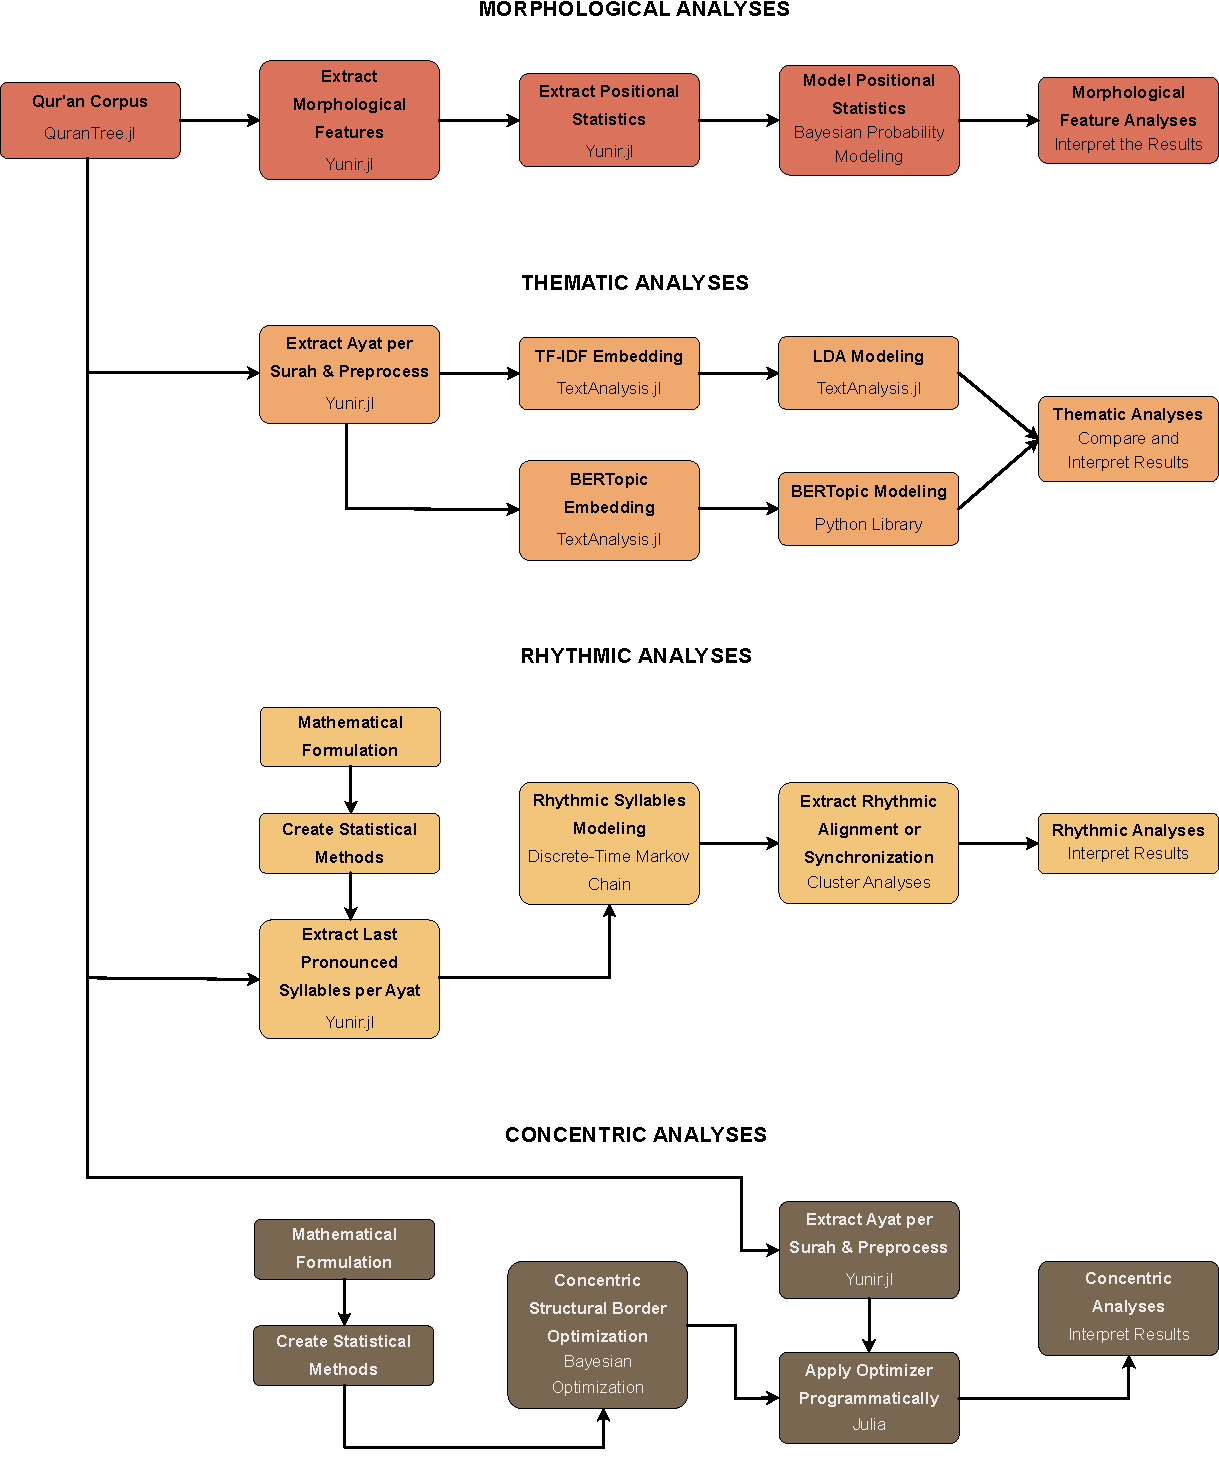
\includegraphics[width=\textwidth]{img/conceptual_framework.pdf}
    \caption{Diagram of Conceptual Framework}
\end{figure}